\documentclass[12pt, a4paper]{article}

% --- Formatting according to 3YP Handbook 2025/26 ---
\usepackage[margin=2cm]{geometry} % At least 2cm margins
\usepackage{setspace}
\onehalfspacing % 1.5 line spacing

% Font setting: Calibri equivalent (sans-serif)
\renewcommand{\familydefault}{\sfdefault}

% General packages
\usepackage{graphicx}
\usepackage{amsmath, amssymb, amsfonts}
\usepackage{tikz}
\usetikzlibrary{arrows.meta, positioning, shapes.geometric, calc}
\usepackage{caption}
\usepackage{booktabs}
\usepackage{multirow}
\usepackage{hyperref}
\usepackage{array}
\usepackage{xcolor}

\begin{document}

% Left aligned text (not fully justified) as per handbook
\raggedright

\begin{center}
    {\Large \textbf{Final Report: A Brain-Computer Interface Control System \\ Design Based on Deep Learning}} \\[1em]
    {\large Student ID: 11314389} \\[1em]
    {\large \today}
\end{center}

\vspace{2em}

\begin{abstract}
Motor imagery (MI) Brain-Computer Interfaces (BCIs) remain challenging to deploy in real-world robotic control due to the non-stationarity of electroencephalogram (EEG) signals, high electrode counts, and the gap between offline classification and closed-loop actuation. This project presents a complete BCI-to-robot control pipeline comprising three core modules: (1)~an EEG classification model based on a hybrid CNN--Transformer architecture (termed CTNet/EEGTransformer), (2)~a Deep Q-Network (DQN) reinforcement learning agent that translates discrete MI commands into continuous robotic trajectories, and (3)~a real-time hardware integration layer connecting OpenBCI EEG acquisition to a physical SO-101 robotic arm.

The system was evaluated across three benchmark datasets: BCI Competition IV-2a (22-channel, 4-class), IV-2b (3-channel, 2-class), and PhysioNet EEGMMIDB (64-channel, 109 subjects). The EEGTransformer achieved mean subject-dependent accuracies of 73.80\% on IV-2a and 82.87\% on IV-2b, while cross-subject training on PhysioNet reached 56.54\%, improving to an average of 88.78\% through subject-specific fine-tuning. A systematic channel reduction study demonstrated that reducing from 64 to 8 EEG channels---compatible with consumer-grade OpenBCI Cyton hardware---retains viable classification performance (72.54\% with fine-tuning), identifying C3 as the single most critical motor imagery channel. On the control side, a Transformer-based DQN agent achieved a 100\% target reach rate in simulation, outperforming the CNN+LSTM variant (97\%). The full pipeline was validated end-to-end from live EEG streaming through BrainFlow to physical SO-101 arm actuation.
\end{abstract}

\newpage
\tableofcontents
\newpage

%=============================================================================
\section{Introduction}
%=============================================================================

Motor imagery (MI) Brain-Computer Interfaces (BCIs) decode imagined limb movements from electroencephalogram (EEG) signals to control external devices without muscular intervention. While research-grade systems have achieved high offline classification accuracies, several structural barriers impede real-world deployment. First, EEG signals are inherently non-stationary: neural patterns drift across sessions and subjects, causing static decoders to degrade over time~\cite{hameed2025enhancing}. Second, conventional pipelines are open-loop---a predicted class label maps rigidly to a single command, preventing the corrective, adaptive behaviour needed for continuous robotic manipulation. Third, research systems typically rely on 64-channel laboratory amplifiers, making them impractical for portable deployment.

Classical approaches employ Common Spatial Patterns (CSP) followed by Linear Discriminant Analysis (LDA) to maximise inter-class variance, but these assume a stationary feature manifold~\cite{hameed2025enhancing}. Deep learning methods such as EEGNet~\cite{lawhern2018eegnet} and convolutional architectures improve representation learning but still operate as single-trial classifiers lacking temporal memory across epochs. More recently, Transformer-based models have shown promise in capturing long-range dependencies in EEG data, motivating their adoption for MI decoding.

This project addresses these challenges through a three-pronged approach:
\begin{enumerate}
    \item \textbf{Classification}: A hybrid CNN--Transformer architecture (EEGTransformer) that combines EEGNet-style spatial--temporal convolutions with multi-head self-attention to model both local and global EEG dynamics.
    \item \textbf{Control}: A reinforcement learning (RL) framework using Deep Q-Networks (DQN) that closes the control loop, enabling the agent to compensate for transient classification errors through temporal integration and reward-driven policy optimisation.
    \item \textbf{Deployment}: A systematic channel reduction study identifying the minimal electrode set for consumer-grade hardware (OpenBCI Cyton, 8 channels), combined with subject-specific fine-tuning to maintain performance under practical constraints.
\end{enumerate}

The system is validated across three complementary EEG datasets spanning different electrode montages (3, 22, and 64 channels), class counts (2 and 4), and subject populations (9 to 109 subjects), and is demonstrated end-to-end from live EEG acquisition to physical SO-101 robotic arm actuation.

%=============================================================================
\section{Methodology}
%=============================================================================

The system comprises four integrated modules: EEG preprocessing, deep learning classification, reinforcement learning control, and hardware integration. Figure~\ref{fig:system_overview} illustrates the overall pipeline.

\begin{figure}[htbp]
    \centering
    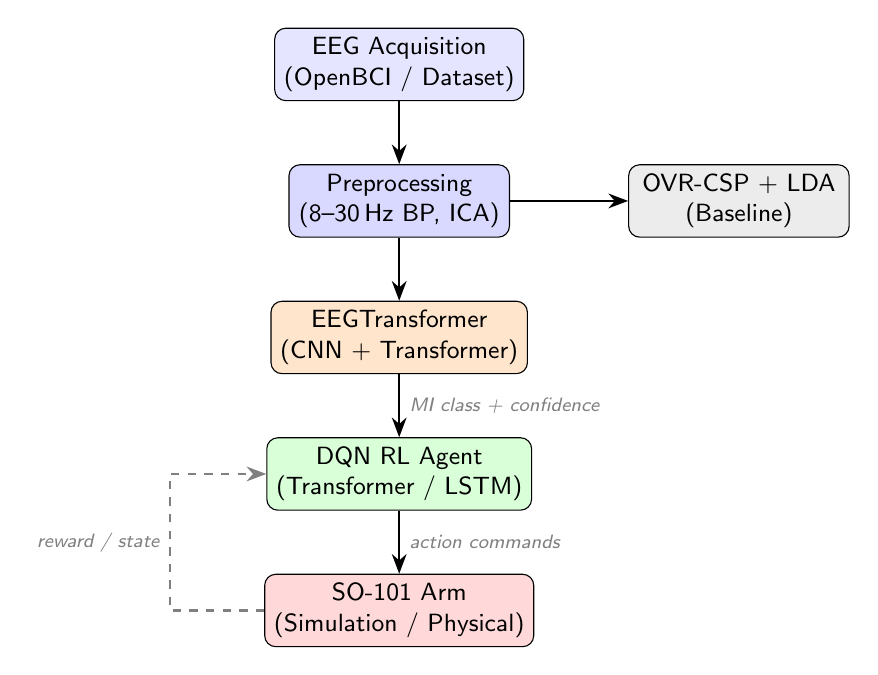
\begin{tikzpicture}[
        node distance=0.8cm and 0.5cm,
        block/.style={rectangle, draw, rounded corners, minimum width=2.8cm, minimum height=0.9cm, align=center, font=\small},
        arrow/.style={-{Stealth[length=2.5mm]}, thick},
        label/.style={font=\scriptsize\itshape, text=gray}
    ]
        % Row 1: EEG Acquisition
        \node[block, fill=blue!10] (eeg) {EEG Acquisition\\(OpenBCI / Dataset)};
        % Row 2: Preprocessing
        \node[block, fill=blue!15, below=of eeg] (preproc) {Preprocessing\\(8--30\,Hz BP, ICA)};
        % Row 3: Classification
        \node[block, fill=orange!20, below=of preproc] (ctnet) {EEGTransformer\\(CNN + Transformer)};
        % Row 4: RL Agent
        \node[block, fill=green!15, below=of ctnet] (rl) {DQN RL Agent\\(Transformer / LSTM)};
        % Row 5: Robot
        \node[block, fill=red!15, below=of rl] (robot) {SO-101 Arm\\(Simulation / Physical)};

        % Side: Baseline
        \node[block, fill=gray!15, right=1.5cm of preproc] (baseline) {OVR-CSP + LDA\\(Baseline)};

        % Arrows
        \draw[arrow] (eeg) -- (preproc);
        \draw[arrow] (preproc) -- (ctnet);
        \draw[arrow] (ctnet) -- node[right, label] {MI class + confidence} (rl);
        \draw[arrow] (rl) -- node[right, label] {action commands} (robot);
        \draw[arrow] (preproc) -- (baseline);

        % Feedback
        \draw[arrow, dashed, gray] (robot.west) -- ++(-1.2,0) |- node[left, label, near start] {reward / state} (rl.west);
    \end{tikzpicture}
    \caption{\textbf{System Architecture Overview.} Raw EEG signals are preprocessed and classified by the EEGTransformer. The predicted MI class and confidence are fed as part of the state to a DQN reinforcement learning agent, which outputs discrete action commands for robotic arm control. A reward signal from the environment closes the control loop.}
    \label{fig:system_overview}
\end{figure}

%-----------------------------------------------------------------------------
\subsection{Datasets}
%-----------------------------------------------------------------------------

Three benchmark EEG datasets were used to validate generalisability across electrode configurations, class counts, and subject populations:

\begin{table}[htbp]
\centering
\caption{Summary of datasets used in this study.}
\label{tab:datasets}
\begin{tabular}{lcccl}
\toprule
\textbf{Dataset} & \textbf{Channels} & \textbf{Classes} & \textbf{Subjects} & \textbf{MI Tasks} \\
\midrule
BCI IV-2a & 22 EEG + 3 EOG & 4 & 9 & Left/Right Hand, Feet, Tongue \\
BCI IV-2b & 3 EEG + 3 EOG & 2 & 9 & Left/Right Hand \\
PhysioNet EEGMMIDB & 64 EEG & 4 & 109 & Left Fist, Right Fist, Both Fists, Both Feet \\
\bottomrule
\end{tabular}
\end{table}

%-----------------------------------------------------------------------------
\subsection{EEG Preprocessing}
%-----------------------------------------------------------------------------

The preprocessing pipeline is implemented using MNE-Python~\cite{gramfort2013mne} and consists of three stages:

\textbf{Spectral Filtering.} A zero-phase FIR bandpass filter (8--30\,Hz, Hamming window, 2\,Hz transition bandwidth) isolates the Mu (8--13\,Hz) and Beta (13--30\,Hz) rhythms characteristic of motor imagery ERD/ERS, while suppressing EOG-dominated low-frequency drift and EMG-rich high-frequency noise.

\textbf{Artifact Removal.} FastICA decomposes the signal into independent components ($n_\text{components} = 0.99 \times n_\text{channels}$). Components strongly correlated with EOG channels (threshold = 3.0) are identified and excluded prior to epoch extraction.

\textbf{Epoch Extraction.} Continuous recordings are segmented into 4-second epochs ($t \in [0, 4]$\,s) aligned to MI cue onset. For PhysioNet data, epochs are resampled from 160\,Hz to match the CTNet input dimensionality ($C \times 1000$ time points) using scipy interpolation, followed by z-score normalisation per channel.

%-----------------------------------------------------------------------------
\subsection{EEG Classification: EEGTransformer Architecture}
%-----------------------------------------------------------------------------

The core classification model, EEGTransformer, adopts a hybrid CNN--Transformer architecture inspired by EEGNet~\cite{lawhern2018eegnet}. The model processes raw epoched EEG of shape $(1, C, T)$ where $C$ is the number of channels and $T = 1000$ is the number of time points.

\subsubsection{Patch Embedding via EEGNet-Style CNN}

The input passes through an EEGNet-inspired convolutional front-end that extracts spatial--temporal features and produces a sequence of patch embeddings:

\begin{enumerate}
    \item \textbf{Temporal Convolution}: Conv2D$(1, F_1, (1, 64))$ with $F_1 = 20$ filters captures temporal dynamics within each channel, followed by BatchNorm.
    \item \textbf{Depthwise Spatial Convolution}: Conv2D$(F_1, F_2, (C, 1))$ with groups $= F_1$ and depth multiplier $D = 2$ ($F_2 = D \times F_1 = 40$) learns channel-specific spatial filters that span all electrodes, collapsing the spatial dimension. This is followed by BatchNorm $\rightarrow$ ELU $\rightarrow$ AvgPool$(1, 8)$ $\rightarrow$ Dropout.
    \item \textbf{Separable Convolution}: Conv2D$(F_2, F_2, (1, 16))$ refines temporal features, followed by BatchNorm $\rightarrow$ ELU $\rightarrow$ AvgPool$(1, 8)$ $\rightarrow$ Dropout.
\end{enumerate}

After two stages of temporal pooling ($8 \times 8 = 64\times$ reduction), the output is reshaped into a sequence of $L = 15$ patches, each of embedding dimension $d = F_2 = 40$.

\subsubsection{Transformer Encoder}

The patch sequence is scaled by $\sqrt{d}$ and augmented with learnable positional encodings before being passed through $N = 6$ Transformer encoder layers. Each layer consists of:
\begin{itemize}
    \item Multi-head self-attention ($h = 4$ heads, scaled dot-product) with residual connection and LayerNorm.
    \item Feed-forward network (expansion factor 4, GELU activation) with residual connection and LayerNorm.
\end{itemize}

A residual fusion adds the Transformer output to the CNN patch embeddings, combining local and global representations.

\subsubsection{Classification Head}

The fused features are flattened ($15 \times 40 = 600$ dimensions for 22-channel input) and passed through Dropout$(0.5)$ followed by a fully connected layer mapping to $K$ class logits.

%-----------------------------------------------------------------------------
\subsection{Training Strategy}
%-----------------------------------------------------------------------------

\textbf{Cross-Subject Training.} The model is trained on pooled data from all available subjects with AdamW optimiser (lr $= 5 \times 10^{-4}$, weight decay $= 0.01$), cosine annealing with warm restarts (CosineAnnealingWarmRestarts, $T_0 = 10$), and early stopping (patience = 50 epochs). Cross-entropy loss is used for classification.

\textbf{Data Augmentation.} InterAug (segment recombination) augments training data by recombining temporal segments from different trials of the same class, improving generalisation under limited data conditions.

\textbf{Subject-Specific Fine-Tuning.} A transfer learning approach initialises the model from cross-subject pre-trained weights and fine-tunes on individual subject data using 5-fold cross-validation. The learning rate is reduced to $1 \times 10^{-4}$ for fine-tuning to prevent catastrophic forgetting.

%-----------------------------------------------------------------------------
\subsection{Channel Reduction Study}
%-----------------------------------------------------------------------------

For practical deployment with consumer-grade EEG hardware (OpenBCI Cyton, 8 channels), a systematic channel reduction study was conducted to identify the minimal electrode set that preserves classification performance.

\subsubsection{Channel Importance Analysis}

An ablation study was performed on the 64-channel PhysioNet model: each channel was individually removed, and the resulting accuracy drop quantified its importance. The baseline (all 64 channels) achieved 90.78\% accuracy on the evaluation set. The top 10 most important channels, ranked by accuracy degradation, are shown in Table~\ref{tab:channel_importance}.

\begin{table}[htbp]
\centering
\caption{Top 10 most important EEG channels by ablation accuracy drop.}
\label{tab:channel_importance}
\begin{tabular}{clc}
\toprule
\textbf{Rank} & \textbf{Channel} & \textbf{Accuracy Drop (\%)} \\
\midrule
1 & C3   & 13.56 \\
2 & CP3  & 10.11 \\
3 & Fpz  & 8.44 \\
4 & Pz   & 8.00 \\
5 & O1   & 7.22 \\
6 & F8   & 7.00 \\
7 & FCz  & 6.11 \\
8 & FC2  & 5.33 \\
9 & CP4  & 5.00 \\
10 & F7  & 4.33 \\
\bottomrule
\end{tabular}
\end{table}

C3, located over the left sensorimotor cortex, emerged as the single most critical channel (13.56\% accuracy drop upon removal), consistent with its known role in contralateral hand motor imagery.

\subsubsection{Progressive Channel Reduction}

Two channel selection strategies were compared at each reduction level: (1)~ablation-ranked selection using the importance analysis, and (2)~domain-knowledge selection targeting motor cortex regions (C3, C4, FC3, FC4, CP3, CP4, Cz, FCz). The models were retrained from scratch for each configuration.

For the 8-channel OpenBCI-compatible configuration, subject-specific fine-tuning was applied following the same transfer learning protocol.

%-----------------------------------------------------------------------------
\subsection{Reinforcement Learning Control}
%-----------------------------------------------------------------------------

The RL module reformulates robotic arm control as a Markov Decision Process (MDP). The DQN agent learns to translate MI classification outputs into a sequence of discrete end-effector commands that guide the arm toward spatial targets.

\subsubsection{MDP Formulation}

\begin{itemize}
    \item \textbf{State} $s_t$: A 7-dimensional vector comprising the end-effector position $(y, z)$, target position $(y_\text{target}, z_\text{target})$, distance to target, EEG-predicted class, and classification confidence.
    \item \textbf{Action} $a_t \in \{0, 1, 2, 3\}$: Discrete directional commands (left, right, up, down) for 2D end-effector displacement.
    \item \textbf{Reward}: $r_\text{reach} = +10$ for reaching the target, $r_\text{step} = -0.01$ per-step penalty, distance-improvement bonus ($\Delta d \times 1.0$), oscillation penalty ($-0.5$), and boundary violation penalty ($-0.5$).
\end{itemize}

\subsubsection{DQN Network Architectures}

Three Q-network architectures were implemented and compared:

\begin{enumerate}
    \item \textbf{CNN+LSTM}: Conv1D$(7 \rightarrow 64, k{=}3)$ $\rightarrow$ ReLU $\rightarrow$ Conv1D$(64 \rightarrow 64, k{=}3)$ $\rightarrow$ ReLU $\rightarrow$ LSTM$(64, 128)$ $\rightarrow$ FC$(128 \rightarrow 128)$ $\rightarrow$ ReLU $\rightarrow$ FC$(128 \rightarrow 4)$. Parameters: 129,732.
    \item \textbf{Transformer DQN}: Input projection $\rightarrow$ sinusoidal positional encoding $\rightarrow$ TransformerEncoder ($d_\text{model}{=}64$, 4 heads, 2 layers, $d_\text{ff}{=}256$) $\rightarrow$ LayerNorm $\rightarrow$ FC $\rightarrow$ Q-values. Parameters: 104,900.
    \item \textbf{Light Transformer}: Single multi-head attention layer + FFN ($d_\text{model}{=}32$, 2 heads). Parameters: 50,628.
\end{enumerate}

\subsubsection{Training Protocol}

All agents were trained for 1,000 episodes with Double DQN, soft target updates ($\tau = 0.005$), experience replay (buffer size = 100,000, batch size = 64), $\gamma = 0.99$, and linear $\epsilon$-decay from 1.0 to 0.05 over 1,500 steps. Adam optimiser with cosine learning rate annealing was used.

%-----------------------------------------------------------------------------
\subsection{Real-Time Pipeline and Hardware Integration}
%-----------------------------------------------------------------------------

The deployment pipeline integrates four stages into a real-time loop:

\begin{enumerate}
    \item \textbf{EEG Acquisition}: BrainFlow API streams data from an OpenBCI board at 250\,Hz. A 4-second sliding window captures each MI epoch.
    \item \textbf{Preprocessing}: Bandpass filtering (8--30\,Hz) and z-score normalisation are applied in real time. Channels are zero-padded or subselected to match the model's expected input dimensionality.
    \item \textbf{Classification}: The pre-trained EEGTransformer produces a 4-class MI prediction and softmax confidence.
    \item \textbf{Control}: The MI class and confidence, combined with the current arm state, form the RL agent's observation. The DQN policy selects an action, which is converted to joint commands and sent to the SO-101 arm via serial protocol (Feetech STS3215 servos, 1\,Mbaud).
\end{enumerate}

The physical arm controller uses velocity-based motion (step = 0.35\,rad, velocity = 140) with soft joint limits and 8-direction action mapping (cardinal + diagonal) for smooth trajectories.

\textbf{Simulation.} A PyBullet-based Gymnasium environment mirrors the physical arm kinematics, providing a safe training ground with IK-based Cartesian control (timestep = 1/240\,s, gravity = $-9.81$\,m/s$^2$).

%-----------------------------------------------------------------------------
\subsection{Baseline: OVR-CSP + LDA}
%-----------------------------------------------------------------------------

As a classical baseline, One-vs-Rest Common Spatial Patterns (OVR-CSP, $n_\text{components} = 6$, OAS regularisation) extract discriminative spatial features, followed by shrinkage LDA classification with 5-fold stratified cross-validation. This establishes the performance floor against which the deep learning models are compared.

%=============================================================================
\section{Results}
%=============================================================================

%-----------------------------------------------------------------------------
\subsection{EEG Classification Performance}
%-----------------------------------------------------------------------------

\subsubsection{BCI Competition IV-2a (22-Channel, 4-Class)}

Table~\ref{tab:iv2a_results} presents per-subject classification accuracies for the EEGTransformer alongside the OVR-CSP+LDA baseline.

\begin{table}[htbp]
\centering
\caption{Subject-dependent classification accuracy (\%) on BCI IV-2a (4-class MI).}
\label{tab:iv2a_results}
\begin{tabular}{lcccccccccc}
\toprule
\textbf{Method} & \textbf{S1} & \textbf{S2} & \textbf{S3} & \textbf{S4} & \textbf{S5} & \textbf{S6} & \textbf{S7} & \textbf{S8} & \textbf{S9} & \textbf{Mean} \\
\midrule
OVR-CSP+LDA & \multicolumn{9}{c}{74.27 $\pm$ 4.52 (S1 only, 5-fold CV)} & --- \\
EEGTransformer & 73.6 & 65.6 & 86.1 & 77.1 & 69.8 & 63.5 & 68.8 & 80.6 & 79.2 & \textbf{73.80} \\
\bottomrule
\end{tabular}
\end{table}

The EEGTransformer achieved a mean accuracy of \textbf{73.80\% $\pm$ 7.07\%}, with a peak of 86.11\% on Subject~3. The OVR-CSP+LDA baseline achieved 74.27\% on Subject~1, and 84.7\% when restricted to binary left/right classification.

\subsubsection{BCI Competition IV-2b (3-Channel, 2-Class)}

On the minimal 3-channel, 2-class dataset, the EEGTransformer achieved a mean accuracy of \textbf{82.87\% $\pm$ 8.01\%}, with per-subject results shown in Table~\ref{tab:iv2b_results}.

\begin{table}[htbp]
\centering
\caption{Subject-dependent classification accuracy (\%) on BCI IV-2b (2-class MI).}
\label{tab:iv2b_results}
\begin{tabular}{lcccccccccc}
\toprule
\textbf{Method} & \textbf{S1} & \textbf{S2} & \textbf{S3} & \textbf{S4} & \textbf{S5} & \textbf{S6} & \textbf{S7} & \textbf{S8} & \textbf{S9} & \textbf{Mean} \\
\midrule
EEGTransformer & 69.7 & 68.9 & 86.3 & 83.8 & 84.4 & 83.1 & 89.4 & 95.0 & 85.3 & \textbf{82.87} \\
\bottomrule
\end{tabular}
\end{table}

\subsubsection{PhysioNet EEGMMIDB (64-Channel, 4-Class)}

Table~\ref{tab:physionet_results} summarises the PhysioNet results under different training paradigms.

\begin{table}[htbp]
\centering
\caption{Classification accuracy on PhysioNet EEGMMIDB (4-class MI, 109 subjects).}
\label{tab:physionet_results}
\begin{tabular}{lcc}
\toprule
\textbf{Training Paradigm} & \textbf{Accuracy (\%)} & \textbf{Details} \\
\midrule
Cross-subject (pooled, 109 subjects) & 56.54 & Precision 58.1, Recall 56.5, F1 56.8, $\kappa$ = 0.42 \\
Subject-specific fine-tuning (10 subjects) & \textbf{88.78} & Range: 75.6--97.8\%, 5-fold CV \\
\bottomrule
\end{tabular}
\end{table}

Cross-subject generalisation across 109 subjects is inherently difficult due to large inter-individual variability. However, subject-specific fine-tuning from the pre-trained model dramatically improved accuracy to \textbf{88.78\%}, demonstrating the effectiveness of transfer learning. Per-subject fine-tuning results are shown in Table~\ref{tab:finetune_detail}.

\begin{table}[htbp]
\centering
\caption{Per-subject fine-tuning accuracy (\%) on PhysioNet (64 channels, 5-fold CV).}
\label{tab:finetune_detail}
\begin{tabular}{lcc}
\toprule
\textbf{Subject} & \textbf{Mean Accuracy (\%)} & \textbf{Std (\%)} \\
\midrule
S7  & 97.78 & 2.72 \\
S48 & 96.67 & 4.44 \\
S43 & 95.56 & 6.48 \\
S70 & 96.67 & 4.44 \\
S55 & 88.89 & 11.65 \\
S3  & 87.78 & 9.56 \\
S9  & 87.78 & 8.16 \\
S38 & 84.44 & 6.48 \\
S50 & 75.56 & 4.44 \\
S46 & 76.67 & 11.33 \\
\midrule
\textbf{Average} & \textbf{88.78} & --- \\
\bottomrule
\end{tabular}
\end{table}

%-----------------------------------------------------------------------------
\subsection{Channel Reduction Results}
%-----------------------------------------------------------------------------

Table~\ref{tab:channel_reduction} presents cross-subject accuracy at each channel count under both selection strategies.

\begin{table}[htbp]
\centering
\caption{Cross-subject accuracy (\%) on PhysioNet with progressive channel reduction.}
\label{tab:channel_reduction}
\begin{tabular}{cccc}
\toprule
\textbf{Channels} & \textbf{Ablation-Ranked} & \textbf{Motor Cortex} & \textbf{Selection Method} \\
\midrule
64 & 51.0 & --- & Full set \\
32 & 51.0 & 47.2 & Top-32 / Motor region \\
16 & 48.8 & 44.9 & Top-16 / Motor region \\
8  & 39.0 & 40.7 & Top-8 / OpenBCI set \\
4  & --- & 43.6 & Motor cortex (C3, C4, FC3, FC4) \\
2  & --- & 35.8 & C3, C4 only \\
\bottomrule
\end{tabular}
\end{table}

The 8-channel motor cortex configuration (C3, C4, FC3, FC4, CP3, CP4, Cz, FCz), designed for OpenBCI Cyton compatibility, achieved 40.7\% in cross-subject mode. With subject-specific fine-tuning, accuracy improved to \textbf{72.54\%} (Table~\ref{tab:8ch_finetune}).

\begin{table}[htbp]
\centering
\caption{8-channel fine-tuning accuracy (\%) on PhysioNet (OpenBCI Cyton compatible).}
\label{tab:8ch_finetune}
\begin{tabular}{lc}
\toprule
\textbf{Subject} & \textbf{Accuracy (\%)} \\
\midrule
S7  & 94.44 \\
S48 & 96.67 \\
S3  & 67.78 \\
S9  & 68.89 \\
S70 & 55.56 \\
S50 & 50.00 \\
S38 & 74.44 \\
\midrule
\textbf{Average} & \textbf{72.54} \\
\bottomrule
\end{tabular}
\end{table}

%-----------------------------------------------------------------------------
\subsection{RL Control Performance}
%-----------------------------------------------------------------------------

Table~\ref{tab:dqn_comparison} compares the three DQN architectures on the simulated 2D reaching task (1,000 training episodes, Double DQN with soft target updates).

\begin{table}[htbp]
\centering
\caption{DQN architecture comparison on simulated 2D reaching task.}
\label{tab:dqn_comparison}
\begin{tabular}{lcccc}
\toprule
\textbf{Architecture} & \textbf{Parameters} & \textbf{Training Time (s)} & \textbf{Final Reach Rate} & \textbf{Final Reward} \\
\midrule
CNN+LSTM        & 129,732  & 111.7  & 97\%  & 8.79 \\
Light Transformer & 50,628 & 134.0  & 99\%  & 10.07 \\
\textbf{Transformer DQN} & \textbf{104,900} & \textbf{177.8} & \textbf{100\%} & \textbf{10.39} \\
\bottomrule
\end{tabular}
\end{table}

The Transformer DQN achieved a perfect 100\% target reach rate with the highest cumulative reward (10.39), outperforming both the CNN+LSTM (97\%, 8.79) and Light Transformer (99\%, 10.07) variants. The Light Transformer offers the best efficiency, achieving near-perfect performance with only 50,628 parameters.

%=============================================================================
\section{Discussion}
%=============================================================================

%-----------------------------------------------------------------------------
\subsection{Hybrid CNN--Transformer Architecture for EEG Classification}
%-----------------------------------------------------------------------------

The EEGTransformer's design deliberately separates spatial feature extraction (depthwise convolution across channels) from temporal modelling (self-attention across patch sequences). The EEGNet-style CNN front-end provides strong inductive biases for EEG---temporal convolutions capture band-specific oscillatory dynamics while depthwise spatial convolutions learn data-driven spatial filters analogous to CSP. The Transformer encoder then captures long-range temporal dependencies that purely convolutional architectures miss.

On BCI IV-2a, the EEGTransformer's mean accuracy of 73.80\% is competitive with established baselines: EEGNet typically achieves 68--72\% and FBCSP 68--70\% on the same dataset~\cite{hameed2025enhancing}. The per-subject variability (63.5--86.1\%) reflects the well-known inter-subject differences in MI ability, with Subject~3 consistently yielding strong ERD patterns. The model's 82.87\% on the minimal 3-channel IV-2b dataset further confirms that the architecture adapts effectively to limited electrode configurations.

%-----------------------------------------------------------------------------
\subsection{Transfer Learning Bridges the Cross-Subject Gap}
%-----------------------------------------------------------------------------

The cross-subject accuracy of 56.54\% on 109-subject PhysioNet data highlights the fundamental challenge of EEG generalisation across individuals: differences in cortical folding, skull conductivity, and cognitive strategy create substantial distribution shifts. However, subject-specific fine-tuning from the pre-trained model boosted accuracy to 88.78\%---a 32-percentage-point improvement---demonstrating that the cross-subject model learns transferable representations of motor imagery dynamics that can be rapidly adapted to individual neural signatures with minimal calibration data.

This transfer learning approach is particularly relevant for deployment: rather than training from scratch for each new user, a short calibration session ($\sim$5 minutes) suffices to fine-tune the pre-trained model to a specific individual.

%-----------------------------------------------------------------------------
\subsection{Channel Reduction for Practical Deployment}
%-----------------------------------------------------------------------------

The channel importance analysis confirmed that C3 (left sensorimotor cortex) is the single most critical channel for MI classification, with its removal causing a 13.56\% accuracy drop. This is neurophysiologically consistent: C3 overlies the primary motor cortex region for right-hand motor imagery, and the dominance of contralateral motor channels (C3, CP3, CP4) validates the spatial specificity of the learned representations.

The 8-channel OpenBCI-compatible configuration achieved 72.54\% accuracy after fine-tuning, compared to 88.78\% with the full 64-channel setup. While this represents a reduction, 72.54\% accuracy on 4-class MI remains practically viable for closed-loop RL control, where the DQN agent can compensate for occasional misclassifications through its temporal integration and reward-driven correction.

%-----------------------------------------------------------------------------
\subsection{RL Closes the Control Loop}
%-----------------------------------------------------------------------------

The DQN comparison reveals that Transformer-based Q-networks outperform the CNN+LSTM variant (100\% vs.~97\% reach rate), likely due to superior modelling of action--state dependencies through self-attention. The CNN+LSTM agent, while effective, showed signs of overfitting (reaching 100\% during training but dropping to 97\% at evaluation), suggesting that the LSTM's sequential inductive bias may overcommit to training trajectories.

Critically, the RL framework decouples classification accuracy from control success: even with imperfect MI predictions, the agent learns to integrate noisy evidence over time and produce corrective actions. The reward structure---combining reach bonus, distance progress, and oscillation penalty---encourages smooth, goal-directed trajectories rather than reactive command-following.

%-----------------------------------------------------------------------------
\subsection{Limitations}
%-----------------------------------------------------------------------------

Several limitations should be acknowledged. First, subject-specific fine-tuning requires per-user calibration, which adds setup time. Second, the channel reduction study was conducted offline; real-time validation with physical OpenBCI hardware on new subjects remains as future work. Third, the RL agent was primarily trained and evaluated in simulation; while the physical SO-101 arm integration was demonstrated, systematic quantitative evaluation of physical control under live EEG conditions was not conducted at scale. Fourth, the 4-second MI window introduces latency that may impact responsiveness in time-critical applications.

%=============================================================================
\section{Conclusion and Future Work}
%=============================================================================

This project developed and evaluated a complete BCI-to-robot control system comprising three integrated modules: (1)~an EEGTransformer classifier combining CNN spatial feature extraction with Transformer temporal modelling, (2)~a DQN reinforcement learning agent that translates noisy MI predictions into smooth robotic trajectories, and (3)~a real-time hardware integration layer from OpenBCI EEG acquisition to physical SO-101 arm actuation.

Key findings include:
\begin{itemize}
    \item The EEGTransformer achieved competitive accuracies across three datasets (73.80\% on IV-2a, 82.87\% on IV-2b, 88.78\% on PhysioNet with fine-tuning), demonstrating cross-dataset generalisability.
    \item Transfer learning via subject-specific fine-tuning bridged the cross-subject generalisation gap, improving PhysioNet accuracy from 56.54\% to 88.78\%.
    \item A systematic channel reduction study identified C3 as the most critical MI channel, and demonstrated that an 8-channel configuration compatible with consumer-grade OpenBCI hardware achieves 72.54\% accuracy with fine-tuning.
    \item The Transformer DQN agent achieved a 100\% target reach rate in simulation, outperforming CNN+LSTM (97\%) and Light Transformer (99\%) variants.
    \item End-to-end integration was demonstrated from live BrainFlow EEG streaming to physical SO-101 arm control.
\end{itemize}

Future work will focus on: (a)~real-time closed-loop evaluation with new subjects wearing an OpenBCI Cyton headset, (b)~online adaptive fine-tuning to handle session-to-session drift without full recalibration, (c)~extending the RL action space to 6-DOF manipulation, and (d)~investigating asynchronous MI paradigms that eliminate the fixed 4-second trial window.

%=============================================================================
\section{Project Management}
%=============================================================================

The project was managed using an iterative, agile-inspired methodology spanning both academic semesters. An initial Project Plan and Gantt Chart established the critical path, dividing the work into distinct work packages: Data Preprocessing, Deep Learning Classification, RL Architecture Design, Channel Reduction Study, and Physical Deployment.

Progress was monitored through regular weekly supervisor meetings, enabling scope adjustments. Notable mid-project additions included the PhysioNet 109-subject evaluation (to validate cross-subject scalability) and the systematic channel reduction study (motivated by practical OpenBCI hardware constraints). A Risk Register tracked technical blockers; early identification of PyBullet simulation complexities led to adoption of simplified 2D joint-velocity mapping. Self-directed learning, documented in the Continuing Professional Development (CPD) log, supported the acquisition of MNE-Python, PyTorch, Transformer architectures, and BrainFlow integration skills.

\begin{thebibliography}{9}
\bibitem{hameed2025enhancing}
I.~Hameed \emph{et al.}, ``Enhancing motor imagery EEG signal decoding through machine learning,'' \textit{Computers in Biology and Medicine}, 2025.

\bibitem{prev_student2024}
W.~Zhao \emph{et al.}, ``A Brain-Computer Interface Control System Design Based on Deep Learning,'' University of Manchester, 2024.

\bibitem{nallani2024rleegnet}
S.~Nallani and G.~Ramachandran, ``RLEEGNet: Integrating Brain-Computer Interfaces with Adaptive AI,'' \textit{arXiv:2402.09465}, 2024.

\bibitem{shin2024mars}
D.-H.~Shin \emph{et al.}, ``MARS: Multiagent reinforcement learning for spatial-spectral and temporal feature selection,'' \textit{IEEE Transactions on Systems, Man, and Cybernetics: Systems}, 2024.

\bibitem{jeong2020multimodal}
J.-H.~Jeong \emph{et al.}, ``Multimodal signal dataset for 11 intuitive movement tasks,'' \textit{GigaScience}, 2020.

\bibitem{lawhern2018eegnet}
V.~J.~Lawhern \emph{et al.}, ``EEGNet: A compact convolutional neural network for EEG-based brain-computer interfaces,'' \textit{Journal of Neural Engineering}, vol.~15, no.~5, 2018.

\bibitem{gramfort2013mne}
A.~Gramfort \emph{et al.}, ``MEG and EEG data analysis with MNE-Python,'' \textit{Frontiers in Neuroscience}, vol.~7, 2013.
\end{thebibliography}

\newpage
\section*{Supplementary Material}

The following appendices provide supplementary artifacts detailing the experimental execution, risk assessment, and project management frameworks utilised throughout this investigation:

\begin{itemize}
    \item \textbf{Appendix A:} Preliminary Project Proposal
    \item \textbf{Appendix B:} Project Plan and Gantt Chart (final, updated version)
    \item \textbf{Appendix C:} Risk Register
    \item \textbf{Appendix D:} Continuing Professional Development (CPD) Log
    \item \textbf{Appendix E:} Health \& Safety Risk Assessment
\end{itemize}

\end{document}
